\documentclass{article}
% Font family
\usepackage{xeCJK}
\setCJKmainfont{Noto Serif TC}
\usepackage{amssymb}
\usepackage{amsmath}

% Document layout
\usepackage[margin=2cm, a4paper]{geometry}
\usepackage{setspace}
\onehalfspacing
\setlength{\parskip}{12pt}
\setlength{\parindent}{0pt}

% Citation
\usepackage{biblatex}
\addbibresource{./ref.bib}

% Image
\usepackage{graphicx}
\graphicspath{{./images/}}

\author{\normalsize 施宇庭 NN6124030}
\date{}


\title{\Large AOC 2024 Spring - Lab 5 AI Compiler}

\begin{document}
\maketitle

\section{Simulation Result}

\begin{figure}[h]
    \centering
    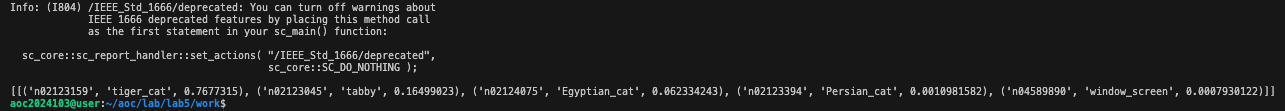
\includegraphics[width=\linewidth]{images/result.png}
\end{figure}

\section{Explain how you tile feature map}

以下解釋如何對 feature maps 做 tiling,重要參數如下:

\begin{itemize}
    \item \verb|tiled_size| (設為 28): 每個 tile 的最大高度和最大寬度
    \item \verb|tiled_stride_h| 和 \verb|tiled_stride_w|: tile 之間的 strides
    \item 每個 tile 最多包含 8 個 channels
\end{itemize}

tiling 以 loop nest 的方式表示如下:

\begin{verbatim}
for (int j = 0; j < padded_h; j += tiled_stride_h) {
    for (int i = 0; i < padded_w; i += tiled_stride_w) {
        // tiled convolution with ifmap channel <= 8, height <= 28, and width <= 28
        // ...
    }
}
\end{verbatim}

tile 的寬和高最大為 28,但不足的部分則是這樣計算:

\begin{verbatim}
int padded_w = ifmap_W + padding_L + padding_R;     // ifmap 經過 padding 後的寬
int padded_h = ifmap_H + padding_T + padding_B;     // ifmap 經過 padding 後的高

int tiled_w = std::min(tiled_size, padded_w - i);
int tiled_h = std::min(tiled_size, padded_h - j);
\end{verbatim}

\section{Explain how you assign DRAM addresses}

\subsection{Weight}

\begin{verbatim}
dram_addr = DRAM_WEIGHT_START_ADDR +
            filter_W * filter_H * ifmap_C * out_c +
            filter_W * filter_H * k;
\end{verbatim}

\verb|out_c| 是第幾個 weight,\verb|k| 則是第幾個 channel

\subsection{Input Feature Map}

\begin{verbatim}
dram_addr = DRAM_INPUT_START_ADDR +
    ifmap_W * ifmap_H * k +
    ifmap_W * (j - !!j) +
    i - !!i;
\end{verbatim}

對 ifmap 來說,\verb|k| 是第幾個 channel,\verb|(j - !!j)| 是 height 方向的 index,\verb|(i - !!i)| 則是 width 方向的 index

當 \verb|i == 0| 時,做一次 NOT 後 \verb|!i| = 1,做兩次 NOT 後 \verb|!!i| = 0,\verb|(i - !!i)| 則會得到 \verb|0 - 0 = 0|。

當 \verb|i != 0| 時,做一次 NOT 後 \verb|!i| = 0,做兩次 NOT 後 \verb|!!i| = 1,\verb|(i - !!i)| 則會得到 \verb|i - 1|。

如此可以確保有 padding 也能取得正確的 addresses,同理 \verb|j| 也可以用同樣的方式計算

\subsection{Output Feature Map}

\begin{verbatim}
dram_addr = DRAM_OUTPUT_START_ADDR +
    ofmap_W * ofmap_H * out_c +
    ofmap_W * j +
    i;
\end{verbatim}

對 ofmap 來說,\verb|out_c| 是第幾個 channel,\verb|j| 是 height 方向的 index,\verb|i| 則是 width 方向的 index

\section{Lesson Learned}

老師上課有講到非常多 AI compiler 的優化技巧,上完課可以理解,但實作上卻較沒有概念,這次 lab 實際動手實作 convolution tiling,讓我們思考 tile 要怎麼切分、遇到 non-perfect size 要怎麼切,還有 DRAM address 的計算,包含 zero-padding 的情況,而這些在期末專題也用得上。

然而,這次 lab 使用較為複雜的 TVM,由於專案規模十分龐大,對新手而言通常會需要非常多時間才能稍微搞懂 compiler 內部的操作,如果可以更有系統性 (由粗到細) 的介紹 TVM 這個框架,應該會對同學入門 AI compiler 很有幫助。

\end{document}
